\documentclass[12pt,addpoints]{repaso}
\grado{1}
\nivel{Secundaria}
\cicloescolar{2024-2025}
\materia{Matemáticas 1 \normalfont \color{darkgray} \\[-0.2em] \small con adecuación curricular a Matemáticas 3$^\circ$ de Primaria.}
\unidad{1, 2 y 3}
\title{Practica la Unidad}
\aprendizajes{\tiny%
      \item Expresa oralmente la sucesión numérica hasta cuatro cifras, en español y hasta donde sea posible, en su lengua materna, de manera ascendente y descendente a partir de un número natural dado.\\[-2em]
      \item Representa, con apoyo de material concreto y modelos gráficos, fracciones: medios, cuartos, octavos, dieciseisavos, para expresar el resultado de mediciones y repartos en situaciones vinculadas a su contexto.\\[-2em]
      \item Resuelve situaciones problemáticas vinculadas a su contexto que implican sumas de números naturales de hasta tres cifras utilizando el algoritmo convencional.\\[-2em]
      \item Resuelve problemas de suma o resta vinculados a su contexto, que impliquen el uso de fracciones (medios, cuartos, octavos, dieciseisavos), con el apoyo de material concreto o representaciones gráficas.\\[-2em]
      \item Resuelve multiplicaciones cuyo producto es un número natural de tres cifras, mediante diversos procedimientos (suma de multiplicaciones parciales, multiplicaciones por 10, 20, 30, entre otros); además, divisiones (reparto y agrupamiento), mediante diversos procedimientos, en particular con la multiplicación; representa la división como: a ÷ b = c.\\[-2em]
      \item A partir de retículas de triángulos, cuadrados o puntos, construye, analiza y clasifica figuras geométricas a partir de sus lados y su simetría, en particular a los triángulos; explica los criterios utilizados para la clasificación.\\[-2em]
      \item Resuelve situaciones problemáticas vinculadas a su contexto que impliquen, medición, estimación y comparación, de longitudes, masas y capacidades, con el uso del metro, kilogramo, litro y medios y cuartos de estas unidades; en el caso de la longitud, el decímetro y centímetro.\\[-2em]
}
\author{Melchor Pinto, JC}
\begin{document}
\INFO
\begin{questions}
	% UNIDAD 1                  
	% \section*{\ifprintanswers{Escritura de cantidades}\else{}\fi}
	% \subsection*{\ifprintanswers{Escritura de cantidades 1 }\else{}\fi}
	% \subsection*{\ifprintanswers{Escritura de cantidades 2 }\else{}\fi}
	% \subsection*{\ifprintanswers{Escritura de cantidades 3 }\else{}\fi}
	% \subsection*{\ifprintanswers{Escritura de cantidades 4 }\else{}\fi}
	% \subsection*{\ifprintanswers{Escritura de cantidades 5 }\else{}\fi}

	\questionboxed[4]{Escribe sore la línea los siguientes números

		\begin{multicols}{2}
			\begin{parts}\large 
            \part \fillin[1849][1.1cm] Mil ochocientos cuarenta y nueve.          
	  			% \part \fillin[1310][1.1cm] Mil trescientos diez.                      
				\part \fillin[ 703][1.1cm] Setecientos tres.                          
				\part \fillin[ 692][1.1cm] Seiscientos noventa y dos.                 
				\part \fillin[ 933][1.1cm] Novecientos treinta y tres.                
				\part \fillin[ 821][1.1cm] Ochocientos veintiuno.                     
				\part \fillin[7269][1.1cm] Siete mil doscientos sesenta y nueve.      
				% \part \fillin[7139][1.1cm] Siete mil ciento treinta y nueve.          
				\part \fillin[8253][1.1cm] Ocho mil doscientos cincuenta y tres.     
				\part \fillin[6724][1.1cm] Seis mil setecientos veinticuatro.    
				% \part \fillin[9205][1.1cm] Nueve mil doscientos cinco.                
				% \part \fillin[5366][1.1cm] Cinco mil trescientos sesenta y seis.      
			\end{parts}
		\end{multicols}
	}
	% \section*{\ifprintanswers{Sistema decimal 1}\else{}\fi}

    % \subsection*{\ifprintanswers{Notación desarrollada 1 }\else{}\fi}
	% \subsection*{\ifprintanswers{Notación desarrollada 2 }\else{}\fi}
	% \subsection*{\ifprintanswers{Notación desarrollada 3 }\else{}\fi}
	
   
	\questionboxed[4]{Escribe la notación desarrollada de cada uno de los siguientes números:

   \begin{multicols}{2}
      \begin{parts}\Large
         \part $15984=$ \fillin[$10000+5000+900+80+4$][2.4in]
         \part $4936 =$ \fillin[$4000+900+30+6$][2.4in]
         \part $27545=$ \fillin[$20000+7000+500+40+5$][2.4in]
         \part $6215 =$ \fillin[$6000+200+10+5$][2.4in]
         \part $5454 =$ \fillin[$5000+400+50+4$][2.4in]
         \part $6451 =$ \fillin[$6000+400+50+1$][2.4in]
         \part $19679=$ \fillin[$10000+9000+600+70+9$][2.4in]
         \part $26324=$ \fillin[$20000+6000+300+20+4$][2.4in]
         \part $5717 =$ \fillin[$5000+700+10+7$][2.4in]
         \part $31126=$ \fillin[$30000+1000+100+20+6$][2.4in]
         \part $4818 =$ \fillin[$4000+800+10+8$][2.4in]
         \part $7145 =$ \fillin[$7000+100+40+5$][2.4in]
      \end{parts}
   \end{multicols}
}
	% \subsection*{\ifprintanswers{Posicionamiento decimal 1 }\else{}\fi}
	% \subsection*{\ifprintanswers{Posicionamiento decimal 2 }\else{}\fi}
	
   \questionboxed[4]{Señala la opción que responda correctamente a cada una de las siguientes preguntas:

		\begin{multicols}{2}
			\begin{parts}\large
				\part ¿Qué lugar ocupa el 6 en 6418?     \fillin[C][0.5cm]
				\part ¿Qué lugar ocupa el 2 en 206418?   \fillin[A][0.5cm]
				\part ¿Qué lugar ocupa el 2 en 87264?    \fillin[D][0.5cm]
				\part ¿Qué lugar ocupa el 1 en 1681?     \fillin[F][0.5cm]
				\part ¿Qué lugar ocupa el 1 en 6138?     \fillin[D][0.5cm]
				\part ¿Qué lugar ocupa el 8 en 198114?   \fillin[C][0.5cm]
				\part ¿Qué lugar ocupa el 7 en 46878?    \fillin[E][0.5cm]
				\part ¿Qué lugar ocupa el 4 en 149778?   \fillin[B][0.5cm]
			\end{parts}

			\columnbreak%

			\begin{choices}\Large
				\choice {\color{red}centenas de millar.}
				\choice {\color{blue}decenas de millar.}
				\choice {\color{Goldenrod}unidades de millar.}
				\choice {\color{red}centenas.}
				\choice {\color{blue}decenas.}
				\choice {\color{Goldenrod}unidades.}
			\end{choices}
		\end{multicols}
	}
   
  
   
   % \section*{\ifprintanswers{Sistema decimal 2}\else{}\fi}
	% \subsection*{\ifprintanswers{Posicionamiento decimal 1 }\else{}\fi}
	% \subsection*{\ifprintanswers{Posicionamiento decimal 2 }\else{}\fi}
	
   \questionboxed[3]{Señala la opción que responda correctamente a cada una de las siguientes preguntas:

		\begin{multicols}{2}
			\begin{parts}\large
				\part En el número 1.829, ¿qué número ocupa la posición de las centésimas?

				\begin{oneparcheckboxes}
					\choice 1 \CorrectChoice 2 \choice 6 \choice 8 \choice 9
				\end{oneparcheckboxes}

				\part En el número 2.087, ¿qué número ocupa la posición de las décimas?

				\begin{oneparcheckboxes}
					\CorrectChoice 0 \choice 2 \choice 7 \choice 8 \choice 9
				\end{oneparcheckboxes}

				\part En el número 5.928, ¿qué número ocupa la posición de las décimas?

				\begin{oneparcheckboxes}
					\choice 5 \choice 2 \choice 6 \choice 8 \CorrectChoice 9
				\end{oneparcheckboxes}

				\part En el número 3.284, ¿qué número ocupa la posición de las milésimas?

				\begin{oneparcheckboxes}
					\choice 2 \choice 3 \CorrectChoice 4  \choice 8 \choice 9
				\end{oneparcheckboxes}

				\part En el número 1.285, ¿qué número ocupa la posición de las décimas?

				\begin{oneparcheckboxes}
					\choice 1 \CorrectChoice 2 \choice 5 \choice 8 \choice 9
				\end{oneparcheckboxes}

				\part En el número 1.823, ¿qué número ocupa la posición de las milésimas?

				\begin{oneparcheckboxes}
					\choice 1 \choice 2 \CorrectChoice 3 \choice 6 \choice 8
				\end{oneparcheckboxes}
			\end{parts}
		\end{multicols}
	}

	\questionboxed[6]{Escribe los siguientes números

		\begin{multicols}{2}
			\begin{parts}\large
				\part Veinticinco enteros ocho décimas                  \\ \hfill \fillin[$25.8$][1cm]
				\part Seis enteros ciento veintiocho milésimas          \\ \hfill \fillin[$6.128$][1cm]
				\part Catorce enteros veintinueve centésimas            \\ \hfill \fillin[$14.29$][1cm]
				\part Cuarenta enteros dos décimas                      \\ \hfill \fillin[$40.2$][1cm]
				\part Tres enteros cincuenta y ocho centésimas          \\ \hfill \fillin[$3.58$][1cm]
				\part Cuatro enteros sesenta y nueve milésimas          \\ \hfill \fillin[$4.069$][1cm]
				\part Siete enteros cuatro décimas                      \\ \hfill \fillin[$ 7.4$][1cm]
				% \part Dos enteros siete décimas                         \\ \hfill \fillin[$2.7$][1cm]
				% \part Cuatro enteros ocho milésimas                     \\ \hfill \fillin[$4.008$][1cm]
				% \part Siete enteros setenta y siete centésimas          \\ \hfill \fillin[$7.77$][1cm]
				% \part Once enteros ochenta y nueve centésimas           \\ \hfill \fillin[$11.89$][1cm]
				\part Treinta y ocho enteros nueve décimas              \\ \hfill \fillin[$38.9$][1cm]
			\end{parts}
		\end{multicols}
	}

   % \subsection*{\ifprintanswers{Notación desarrollada 1 }\else{}\fi}
	% \subsection*{\ifprintanswers{Notación desarrollada 2  }\else{}\fi}
	% \subsection*{\ifprintanswers{Posicionamiento decimal y Notación desarrollada }\else{}\fi}
	
   \questionboxed[4]{Señala la opción que responda correctamente a cada una de las siguientes preguntas:

   \begin{multicols}{2}
      \begin{parts}\large
         \part En el número 3658, ¿qué número ocupa la posición de las decenas?

         \begin{oneparcheckboxes}
            \choice 3 \CorrectChoice 5 \choice 6 \choice 8 \choice 9
         \end{oneparcheckboxes}

         \part En el número 17542, ¿qué número ocupa la posición de las unidades de millar?

         \begin{oneparcheckboxes}
            \choice 1 \CorrectChoice 7 \choice 5 \choice 4 \choice 2
         \end{oneparcheckboxes}

         \part En el número 5984, ¿qué número ocupa la posición de las centenas?

         \begin{oneparcheckboxes}
            \choice 4 \choice 2 \choice 5 \choice 8 \CorrectChoice 9
         \end{oneparcheckboxes}

         \part En el número 7841, ¿qué número ocupa la posición de las decenas?

         \begin{oneparcheckboxes}
            \choice 1 \choice 7 \choice 8 \CorrectChoice 4 \choice 2
         \end{oneparcheckboxes}

         \part En el número 3918, ¿qué número ocupa la posición de las centenas?

         \begin{oneparcheckboxes}
            \choice 3 \choice 1 \choice 6 \choice 8 \CorrectChoice 9
         \end{oneparcheckboxes}

         \part En el número 3621, ¿qué número ocupa la posición de las decenas?

         \begin{oneparcheckboxes}
            \CorrectChoice 2 \choice 3 \choice 6 \choice 8 \choice 1
         \end{oneparcheckboxes}

         \part En el número 51362, ¿qué número ocupa la posición de las decenas de millar?

         \begin{oneparcheckboxes}
            \choice 3 \CorrectChoice 5 \choice 6 \choice 1 \choice 2
         \end{oneparcheckboxes}

         \part En el número 7584, ¿qué número ocupa la posición de las decenas?

         \begin{oneparcheckboxes}
            \choice 3 \choice 5 \choice 7 \CorrectChoice 8 \choice 4
         \end{oneparcheckboxes}

         % \part En el número 9654, ¿qué número ocupa la posición de las centenas?

         % \begin{oneparcheckboxes}
         %    \choice 3 \choice 5 \CorrectChoice 6 \choice 4 \choice 9
         % \end{oneparcheckboxes}

         % \part En el número 240679, ¿qué número ocupa la posición de las centenas de millar?

         % \begin{oneparcheckboxes}
         %    \choice 0 \choice 6 \CorrectChoice 2 \choice 7 \choice 9 \choice 4
         % \end{oneparcheckboxes}
         % \part En el número 41589, ¿qué número ocupa la posición de las decenas de millar?
         % \part En el número 8459, ¿qué número ocupa la posición de las centenas?
         % \part En el número 10562, ¿qué número ocupa la posición de las centenas?
         % \part En el número 24781, ¿qué número ocupa la posición de las decenas de millar?
         % \part En el número 7856, ¿qué número ocupa la posición de las decenas?
      \end{parts}
   \end{multicols}
}

   % \section*{\ifprintanswers{Tablas de multiplicar 1}\else{}\fi}
	% \subsection*{\ifprintanswers{Tabla del 1  }\else{}\fi}
	% \subsection*{\ifprintanswers{Tabla del 2 }\else{}\fi}
	% \subsection*{\ifprintanswers{Tabla del 3 }\else{}\fi}
	% \subsection*{\ifprintanswers{Tabla del 4 }\else{}\fi}
	% \subsection*{\ifprintanswers{Tabla del 5 }\else{}\fi}

	% UNIDAD 2

	% \section*{\ifprintanswers{Tablas de multiplicar 2        }\else{}\fi}
	% \subsection*{\ifprintanswers{Tabla del 6                    }\else{}\fi}
	% \subsection*{\ifprintanswers{Tabla del 7                    }\else{}\fi}
	% \subsection*{\ifprintanswers{Tabla del 8                    }\else{}\fi}
	% \subsection*{\ifprintanswers{Tabla del 9                    }\else{}\fi}
	% \subsection*{\ifprintanswers{Tabla del 10                   }\else{}\fi}
	
   \questionboxed[8]{Reponde las siguientes tablas de multiplicar:

		\begin{multicols}{4}
			\begin{parts}\Large
				\part $5 \times 9=$ \fillin[$45$][0cm]
				\part $5 \times 6=$ \fillin[$30$][0cm]
				\part $6 \times 8=$ \fillin[$48$][0cm]
				\part $6 \times 9=$ \fillin[$54$][0cm]
				\part $3 \times 6=$ \fillin[$18$][0cm]
				\part $2 \times 7=$ \fillin[$14$][0cm]
				\part $4 \times 7=$ \fillin[$28$][0cm]
				\part $3 \times 8=$ \fillin[$24$][0cm]
				\part $2 \times 9=$ \fillin[$18$][0cm]
				\part $4 \times 4=$ \fillin[$16$][0cm]
				\part $7 \times 7=$ \fillin[$49$][0cm]
				\part $7 \times 5=$ \fillin[$35$][0cm]
				\part $5 \times 4=$ \fillin[$20$][0cm]
				\part $8 \times 7=$ \fillin[$56$][0cm]
				\part $7 \times 6=$ \fillin[$42$][0cm]
				\part $9 \times 7=$ \fillin[$63$][0cm]
			\end{parts}
		\end{multicols}
	}

	\questionboxed[8]{Completa las siguientes tablas de multiplicar:

		\begin{multicols}{4}
			\begin{parts}\Large
				\part $\fillin[6][0.5cm] \times 6= 36$
				\part $\fillin[8][0.5cm] \times 8= 64$
				\part $\fillin[7][0.5cm] \times 8= 56$
				\part $5 \times \fillin[10][0.5cm]=50$
				\part $4 \times \fillin[8][0.5cm]=32$
				\part $8 \times \fillin[5][0.5cm]= 40$
				\part $\fillin[6][0.5cm] \times 4= 24$
				\part $7 \times \fillin[7][0.5cm]= 49$
				\part $\fillin[8][0.5cm] \times 3= 24$
				\part $9 \times \fillin[8][0.5cm]= 72$
				\part $\fillin[9][0.5cm] \times 5= 45$
				\part $6 \times \fillin[7][0.5cm]= 42$
				\part $\fillin[9][0.5cm] \times 9= 81$
				\part $4 \times \fillin[9][0.5cm]= 36$
				\part $\fillin[7][0.5cm] \times 4= 28$
				\part $\fillin[9][0.5cm] \times 3= 21$
			\end{parts}
		\end{multicols}
	}
   
   % \section*{\ifprintanswers{Sumas 1                        }\else{}\fi}
	% \subsection*{\ifprintanswers{Sumando con 1, 2 y 3           }\else{}\fi}
	% \subsection*{\ifprintanswers{Sumando con 4, 5 y 6           }\else{}\fi}
	% \subsection*{\ifprintanswers{Sumando con 7, 8 y 9           }\else{}\fi}
	% \subsection*{\ifprintanswers{Sumando números entre 10 y 20  }\else{}\fi}
	% \subsection*{\ifprintanswers{Sumando números entre 20 y 50  }\else{}\fi}
	
   % \section*{\ifprintanswers{Sumas 2                        }\else{}\fi}
	% \subsection*{\ifprintanswers{Sumas hasta el 100             }\else{}\fi}
	% \subsection*{\ifprintanswers{Sumas hasta el 500             }\else{}\fi}
	% \subsection*{\ifprintanswers{Sumas con acarreos 1           }\else{}\fi}
	% \subsection*{\ifprintanswers{Sumas con acarreos 2           }\else{}\fi}
	% \subsection*{\ifprintanswers{Sumas con acarreos 3           }\else{}\fi}
	
   \questionboxed[8]{Realiza las siguientes sumas:

		\begin{multicols}{4}
			\begin{parts}
				\part \ifprintanswers{\large  \quad   \opadd[hfactor=decimal,resultstyle=\color{red},carryadd=true,carrysub=false]{37854}{18581} }
				\else{          \large  \quad  \opadd[hfactor=decimal,resultstyle=\color{white},carryadd=false,carrysub=false]{37854}{18581} }
				\fi
				\part \ifprintanswers{\large  \quad   \opadd[hfactor=decimal,resultstyle=\color{red},carryadd=true,carrysub=false]{3234}{24156} }
				\else{          \large  \quad  \opadd[hfactor=decimal,resultstyle=\color{white},carryadd=false,carrysub=false]{3234}{24156} }
				\fi
				\part \ifprintanswers{\large  \quad   \opadd[hfactor=decimal,resultstyle=\color{red},carryadd=true,carrysub=false]{30985}{19562} }
				\else{          \large  \quad  \opadd[hfactor=decimal,resultstyle=\color{white},carryadd=false,carrysub=false]{30985}{19562} }
				\fi
				\part \ifprintanswers{\large  \quad   \opadd[hfactor=decimal,resultstyle=\color{red},carryadd=true,carrysub=false]{2849}{2415} }
				\else{          \large  \quad  \opadd[hfactor=decimal,resultstyle=\color{white},carryadd=false,carrysub=false]{2849}{2415} }
				\fi
				\part \ifprintanswers{\large  \quad   \opadd[hfactor=decimal,resultstyle=\color{red},carryadd=true,carrysub=false]{31085}{19001} }
				\else{          \large  \quad  \opadd[hfactor=decimal,resultstyle=\color{white},carryadd=false,carrysub=false]{31085}{19001} }
				\fi
				\part \ifprintanswers{\large  \quad   \opadd[hfactor=decimal,resultstyle=\color{red},carryadd=true,carrysub=false]{35701}{25484} }
				\else{          \large  \quad  \opadd[hfactor=decimal,resultstyle=\color{white},carryadd=false,carrysub=false]{35701}{25484} }
				\fi
				\part \ifprintanswers{\large  \quad   \opadd[hfactor=decimal,resultstyle=\color{red},carryadd=true,carrysub=false]{45668}{19624} }
				\else{          \large  \quad  \opadd[hfactor=decimal,resultstyle=\color{white},carryadd=false,carrysub=false]{45668}{19624} }
				\fi
				\part \ifprintanswers{\large  \quad   \opadd[hfactor=decimal,resultstyle=\color{red},carryadd=true,carrysub=false]{58718}{3652} }
				\else{          \large  \quad  \opadd[hfactor=decimal,resultstyle=\color{white},carryadd=false,carrysub=false]{58718}{3652} }
				\fi
			\end{parts}
		\end{multicols}
	}
   
   % \section*{\ifprintanswers{Restas 1                       }\else{}\fi}
	% \subsection*{\ifprintanswers{Restando con 1, 2 y 3          }\else{}\fi}
	% \subsection*{\ifprintanswers{Restando con 4, 5, 6, 7, 8 y 9 }\else{}\fi}
	% \subsection*{\ifprintanswers{Restas como sumas 1            }\else{}\fi}
	% \subsection*{\ifprintanswers{Restas como suma 2             }\else{}\fi}
	% \subsection*{\ifprintanswers{Restas como suma 3             }\else{}\fi}
	
   
   % \section*{\ifprintanswers{Restas 2                       }\else{}\fi}
	% \subsection*{\ifprintanswers{Restas sin transformación 1    }\else{}\fi}
	% \subsection*{\ifprintanswers{Restas sin transformación 2    }\else{}\fi}
	% \subsection*{\ifprintanswers{Restas con transformación 1    }\else{}\fi}
	% \subsection*{\ifprintanswers{Restas con transformación 2    }\else{}\fi}
	% \subsection*{\ifprintanswers{Restas con transformación 3    }\else{}\fi}

   \questionboxed[8]{Realiza las siguientes restas:

		\begin{multicols}{4}
			\begin{parts}
				\part \ifprintanswers{\large  \quad   \opsub[hfactor=decimal,resultstyle=\color{red},carryadd=true,carrysub=true]{4000}{2267} }
				\else{          \large  \quad  \opsub[hfactor=decimal,resultstyle=\color{white},carryadd=false,carrysub=false]{4000}{2267} }
				\fi
				\part \ifprintanswers{\large  \quad   \opsub[hfactor=decimal,resultstyle=\color{red},carryadd=true,carrysub=true]{800}{744} }
				\else{          \large  \quad  \opsub[hfactor=decimal,resultstyle=\color{white},carryadd=false,carrysub=false]{800}{744} }
				\fi
				\part \ifprintanswers{\large  \quad   \opsub[hfactor=decimal,resultstyle=\color{red},carryadd=true,carrysub=true]{3500}{308} }
				\else{          \large  \quad  \opsub[hfactor=decimal,resultstyle=\color{white},carryadd=false,carrysub=false]{3500}{308} }
				\fi
				\part \ifprintanswers{\large  \quad   \opsub[hfactor=decimal,resultstyle=\color{red},carryadd=true,carrysub=true]{3000}{189} }
				\else{          \large  \quad  \opsub[hfactor=decimal,resultstyle=\color{white},carryadd=false,carrysub=false]{3000}{189} }
				\fi
				\part \ifprintanswers{\large  \quad   \opsub[hfactor=decimal,resultstyle=\color{red},carryadd=true,carrysub=true]{1200}{966} }
				\else{          \large  \quad  \opsub[hfactor=decimal,resultstyle=\color{white},carryadd=false,carrysub=false]{1200}{966} }
				\fi
				\part \ifprintanswers{\large  \quad   \opsub[hfactor=decimal,resultstyle=\color{red},carryadd=true,carrysub=true]{3300}{2117} }
				\else{          \large  \quad  \opsub[hfactor=decimal,resultstyle=\color{white},carryadd=false,carrysub=false]{3300}{2117} }
				\fi
				\part \ifprintanswers{\large  \quad   \opsub[hfactor=decimal,resultstyle=\color{red},carryadd=true,carrysub=true]{2000}{1251} }
				\else{          \large  \quad  \opsub[hfactor=decimal,resultstyle=\color{white},carryadd=false,carrysub=false]{2000}{1251} }
				\fi
				\part \ifprintanswers{\large  \quad   \opsub[hfactor=decimal,resultstyle=\color{red},carryadd=true,carrysub=true]{2400}{2023} }
				\else{          \large  \quad  \opsub[hfactor=decimal,resultstyle=\color{white},carryadd=false,carrysub=false]{2400}{2023} }
				\fi
				% \part \ifprintanswers{\large  \quad   \opsub[hfactor=decimal,resultstyle=\color{red},carryadd=true,carrysub=false]{2400}{211} }
				% \else{          \large  \quad  \opsub[hfactor=decimal,resultstyle=\color{white},carryadd=false,carrysub=false]{2400}{211} }
				% \fi
				% \part \ifprintanswers{\large  \quad   \opsub[hfactor=decimal,resultstyle=\color{red},carryadd=true,carrysub=false]{1500}{1044} }
				% \else{          \large  \quad  \opsub[hfactor=decimal,resultstyle=\color{white},carryadd=false,carrysub=false]{1500}{1044} }
				% \fi
				% \part \ifprintanswers{\large  \quad   \opsub[hfactor=decimal,resultstyle=\color{red},carryadd=true,carrysub=false]{2000}{1105} }
				% \else{          \large  \quad  \opsub[hfactor=decimal,resultstyle=\color{white},carryadd=false,carrysub=false]{2000}{1105} }
				% \fi
				% \part \ifprintanswers{\large  \quad   \opsub[hfactor=decimal,resultstyle=\color{red},carryadd=true,carrysub=false]{1600}{669} }
				% \else{          \large  \quad  \opsub[hfactor=decimal,resultstyle=\color{white},carryadd=false,carrysub=false]{1600}{669} }
				% \fi
			\end{parts}
		\end{multicols}
	}

	% UNIDAD 3

	% \section*{\ifprintanswers{Restas 3                                   }\else{}\fi}
	% \subsection*{\ifprintanswers{Restas con transformación 1                }\else{}\fi}
	% \subsection*{\ifprintanswers{Restas con transformación 2                }\else{}\fi}
	% \subsection*{\ifprintanswers{Minuendos múltiplos de 10                  }\else{}\fi}
	% \subsection*{\ifprintanswers{Minuendos con ceros intermedios            }\else{}\fi}
	% \subsection*{\ifprintanswers{Repaso de restas                           }\else{}\fi}
	
   
   % \section*{\ifprintanswers{Multiplicaciones                           }\else{}\fi}
	% \subsection*{\ifprintanswers{Multiplicaciones con una cifra 1           }\else{}\fi}
	% \subsection*{\ifprintanswers{Multiplicaciones con una cifra 2           }\else{}\fi}
	% \subsection*{\ifprintanswers{Multiplicaciones con una cifra 3           }\else{}\fi}
	% \subsection*{\ifprintanswers{Multiplicaciones con una cifra 4           }\else{}\fi}
	% \subsection*{\ifprintanswers{Multiplicaciones con dos cifras            }\else{}\fi}
	
   \questionboxed[6]{Realiza las siguientes multiplicaciones:

		\begin{multicols}{3}
			\begin{parts}
				\part \ifprintanswers{\large  \quad   \opmul[hfactor=decimal,resultstyle=\color{red},displayintermediary=None]{314}{2} }
				\else{          \large  \quad  \opmul[hfactor=decimal,resultstyle=\color{white},displayintermediary=None]{314}{2} }
				\fi
				\part \ifprintanswers{\large  \quad   \opmul[hfactor=decimal,resultstyle=\color{red},displayintermediary=None]{283}{4} }
				\else{          \large  \quad  \opmul[hfactor=decimal,resultstyle=\color{white},displayintermediary=None]{283}{4} }
				\fi
				\part \ifprintanswers{\large  \quad   \opmul[hfactor=decimal,resultstyle=\color{red},displayintermediary=None]{2781}{5} }
				\else{          \large  \quad  \opmul[hfactor=decimal,resultstyle=\color{white},displayintermediary=None]{2781}{5} }
				\fi
				\part \ifprintanswers{\large  \quad   \opmul[hfactor=decimal,resultstyle=\color{red},displayintermediary=None]{4914}{6} }
				\else{          \large  \quad  \opmul[hfactor=decimal,resultstyle=\color{white},displayintermediary=None]{4914}{6} }
				\fi
				\part \ifprintanswers{\large  \quad   \opmul[hfactor=decimal,resultstyle=\color{red},displayintermediary=None]{255}{24} }
				\else{          \large  \quad  \opmul[hfactor=decimal,resultstyle=\color{white},displayintermediary=None]{255}{24} }
				\fi
				\part \ifprintanswers{\large  \quad   \opmul[hfactor=decimal,resultstyle=\color{red},displayintermediary=None]{3533}{29} }
				\else{          \large  \quad  \opmul[hfactor=decimal,resultstyle=\color{white},displayintermediary=None]{3533}{29} }
				\fi
			\end{parts}
		\end{multicols}
	}

   
   % \section*{\ifprintanswers{Divisiones                                 }\else{}\fi}
	% \subsection*{\ifprintanswers{Divisiones del 1 al 5                      }\else{}\fi}
	% \subsection*{\ifprintanswers{Divisiones del 6 al 10                     }\else{}\fi}
	% \subsection*{\ifprintanswers{Divisiones sin residuos                    }\else{}\fi}
	% \subsection*{\ifprintanswers{Divisiones con residuo 1                   }\else{}\fi}
	% \subsection*{\ifprintanswers{Divisiones con residuo 2                   }\else{}\fi}

   \questionboxed[8]{Realiza las siguientes divisiones:

   \begin{multicols}{4}
      \begin{parts}
         \part \ifprintanswers{\large\opidiv{123}{6}} \\[1em]
         \else{          \Large  \quad $6 \overline{) \ 123\ }$} \\[2em]
         \fi

         \part \ifprintanswers{\large\opidiv{200}{3}} \\[1em]
         \else{          \Large  \quad $3 \overline{) \ 200\ }$} \\[2em]
         \fi

         \part \ifprintanswers{\large\opidiv{399}{8}} \\[1em]
         \else{          \Large  \quad $8 \overline{) \ 399\ }$} \\[2em]
         \fi

         \part \ifprintanswers{\large\opidiv{193}{7}} \\[1em]
         \else{          \Large  \quad $7 \overline{) \ 193\ }$} \\[2em]
         \fi

         \part \ifprintanswers{\large\opidiv{283}{6}} \\[1em]
         \else{          \Large  \quad $6 \overline{) \ 283\ }$} \\[2em]
         \fi

         \part \ifprintanswers{\large\opidiv{432}{9}} \\[1em]
         \else{          \Large  \quad $9 \overline{) \ 432\ }$} \\[2em]
         \fi

         \part \ifprintanswers{\large\opidiv{644}{8}} \\[1em]
         \else{          \Large  \quad $8 \overline{) \ 644\ }$} \\[2em]
         \fi

         \part \ifprintanswers{\large\opidiv{656}{7}} \\[1em]
         \else{          \Large  \quad $7 \overline{) \ 656\ }$} \\[2em]
         \fi
      \end{parts}
   \end{multicols}
}

   % \section*{\ifprintanswers{Introducción a las fracciones              }\else{}\fi}
	% \subsection*{\ifprintanswers{Clasificación de fracciones                }\else{}\fi}
	
   \questionboxed[5]{Clasifica las siguientes fracciones en propias, impropias o mixtas:

		\begin{multicols}{5}
			\begin{parts}\large
				\part $\dfrac{5}{6}$   \fillin[Propia][1.5cm]   \\[1em]
				\part $5\dfrac{5}{11}$ \fillin[Mixta][1.5cm]    \\[1em]
				\part $\dfrac{7}{3}$   \fillin[Impropia][1.5cm] \\[1em]
				\part $\dfrac{3}{4}$   \fillin[Propia][1.5cm]   \\[1em]
				\part $1\dfrac{2}{3}$  \fillin[Mixta][1.5cm]    \\[1em]
				\part $\dfrac{7}{5}$   \fillin[Impropia][1.5cm] \\[1em]
				\part $\dfrac{7}{8}$   \fillin[Propia][1.5cm]   \\[1em]
				\part $3\dfrac{2}{9}$  \fillin[Mixta][1.5cm]    \\[1em]
				\part $\dfrac{3}{2}$   \fillin[Impropia][1.5cm] \\[1em]
				 \part $4\dfrac{1}{4}=$ \fillin[Mixta][1.5cm]   \\[1em]
			\end{parts}
		\end{multicols}
	}
   
   % \subsection*{\ifprintanswers{Representación de fracciones               }\else{}\fi}
	
   \questionboxed[5]{Escribe sobre la línea la fracción que representa cada imagen:

		\begin{multicols}{5}
			\begin{parts}
				\part 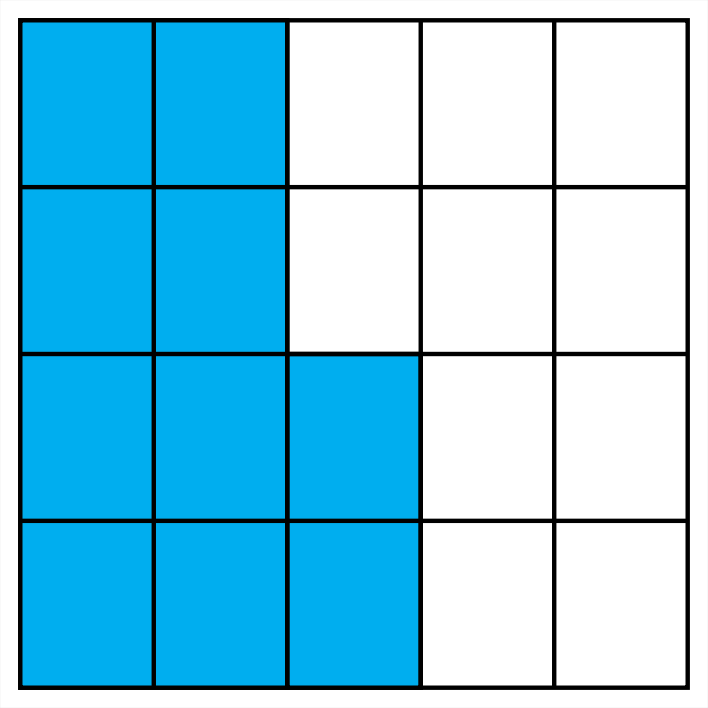
\includegraphics[width=45px]{../images/imagen_frac01.png} \fillin[\fbox{$\dfrac{10}{20}$}][0in] \\[1em]
				\part 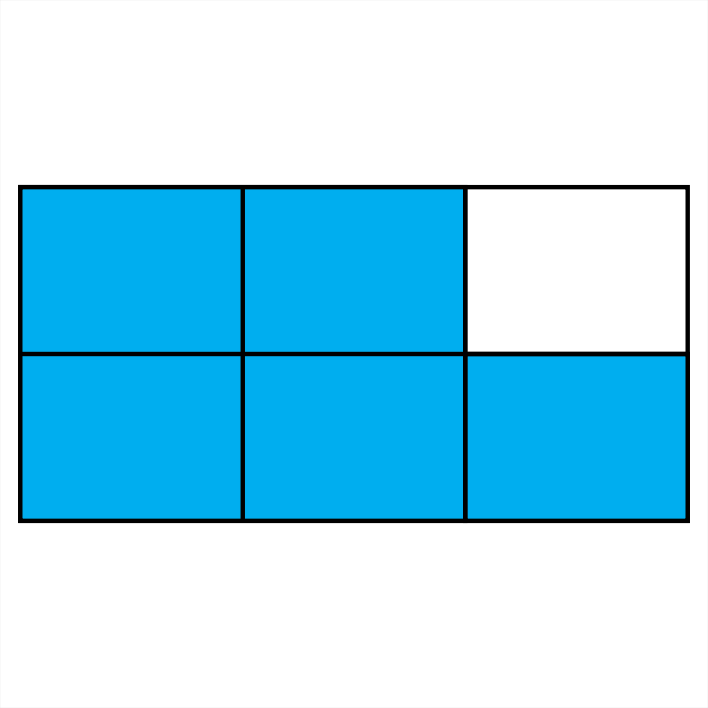
\includegraphics[width=45px]{../images/imagen_frac02.png} \fillin[\fbox{$\dfrac{5}{6}$}][0in] \\[1em]
				\part 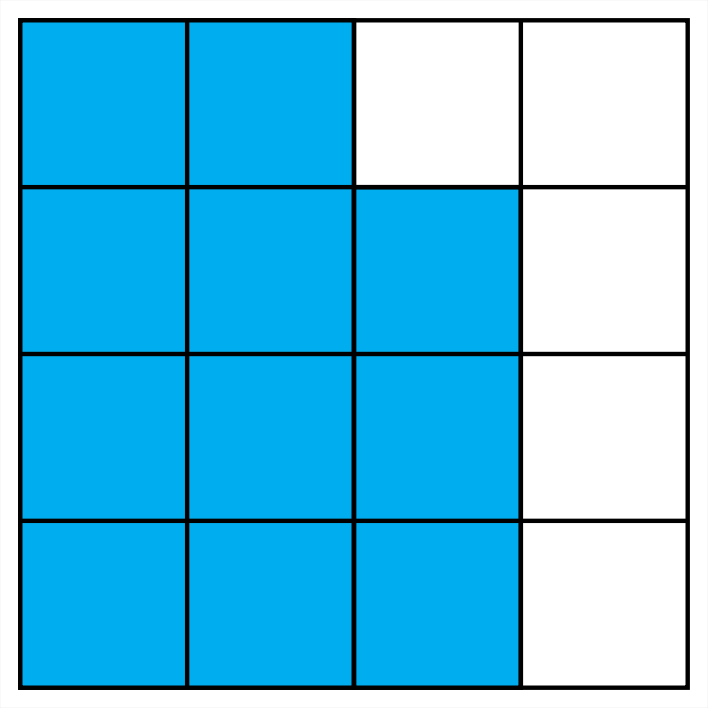
\includegraphics[width=45px]{../images/imagen_frac03.png} \fillin[\fbox{$\dfrac{11}{16}$}][0in] \\[1em]
				\part 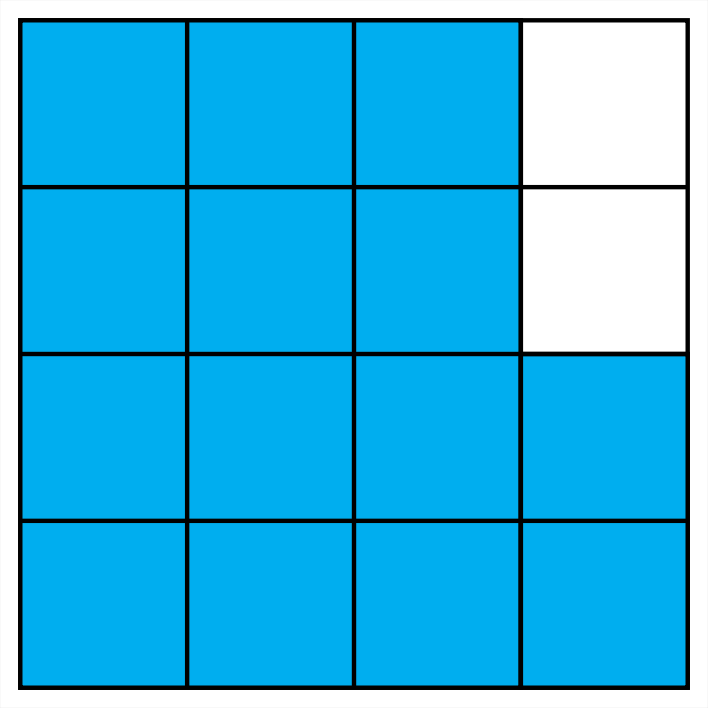
\includegraphics[width=45px]{../images/imagen_frac04.png} \fillin[\fbox{$\dfrac{14}{16}$}][0in] \\[1em]
				\part 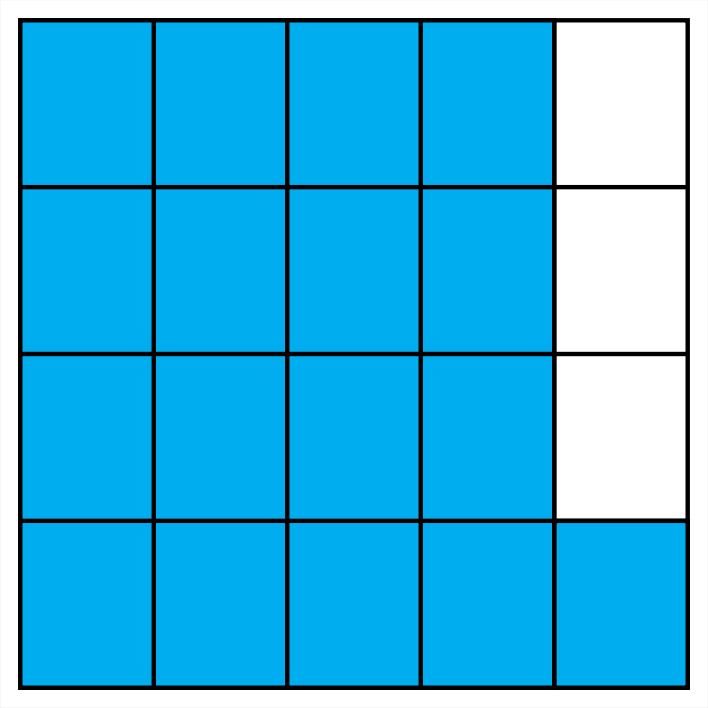
\includegraphics[width=45px]{../images/imagen_frac05.png} \fillin[\fbox{$\dfrac{17}{20}$}][0in] \\[1em]
				\part 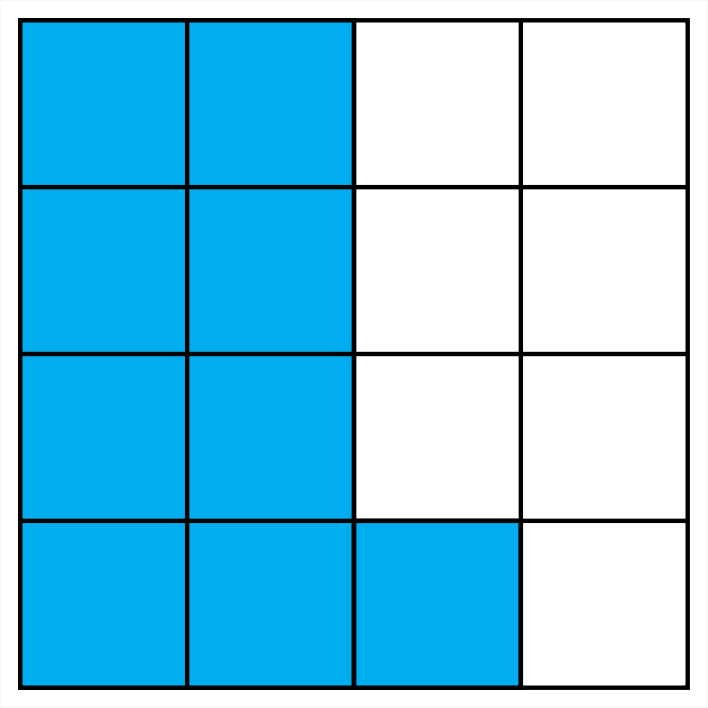
\includegraphics[width=45px]{../images/imagen_frac06.png} \fillin[\fbox{$\dfrac{9}{16}$}][0in] \\[1em]
				\part 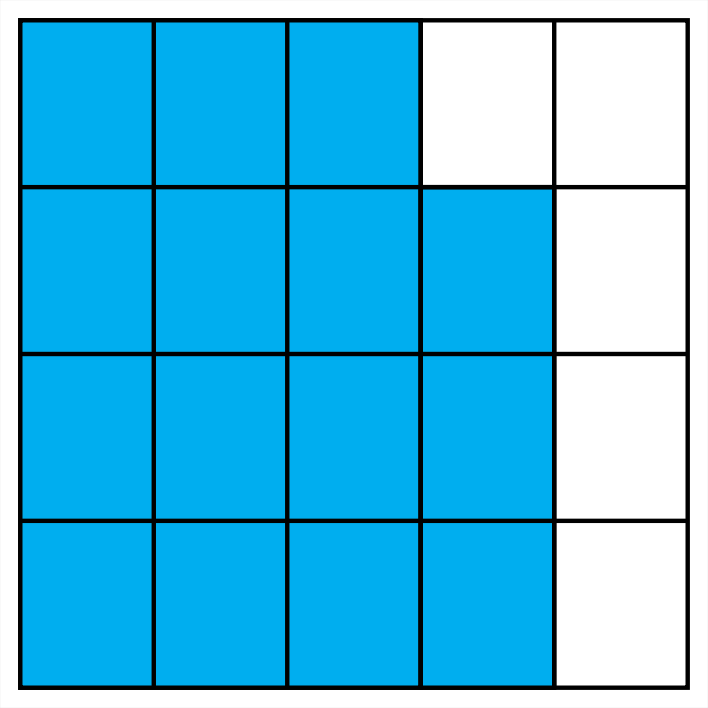
\includegraphics[width=45px]{../images/imagen_frac07.png} \fillin[\fbox{$\dfrac{15}{20}$}][0in] \\[1em]
				\part 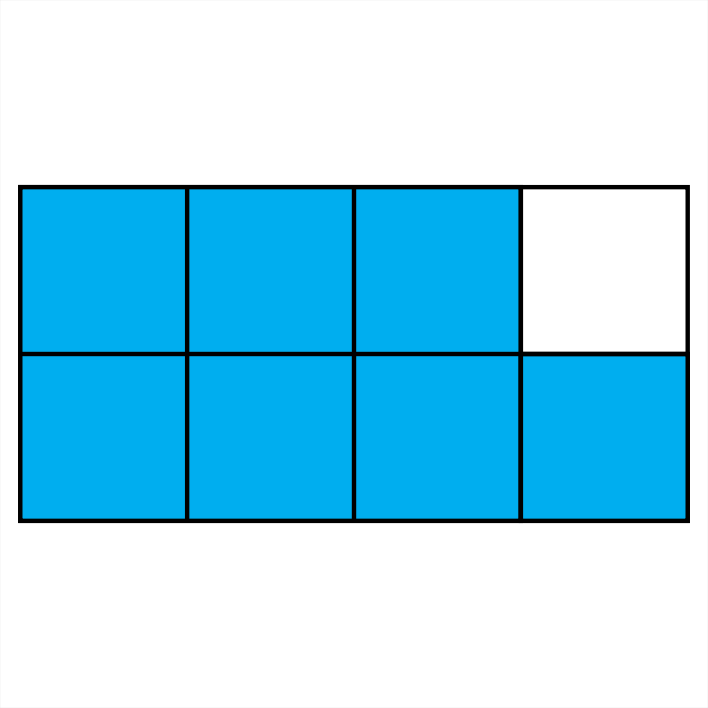
\includegraphics[width=45px]{../images/imagen_frac08.png} \fillin[\fbox{$\dfrac{7}{8}$}][0in] \\[1em]
				\part 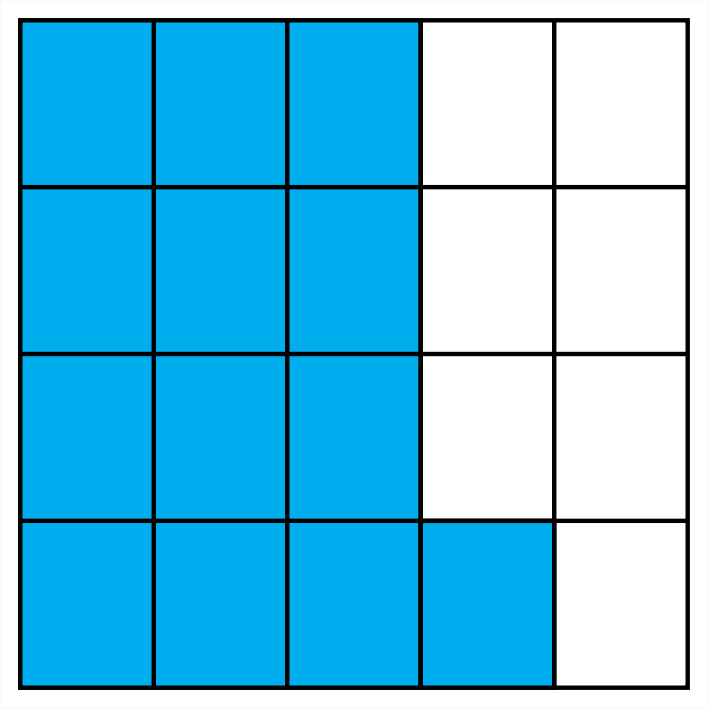
\includegraphics[width=45px]{../images/imagen_frac09.png} \fillin[\fbox{$\dfrac{13}{20}$}][0in] \\[1em]
				\part 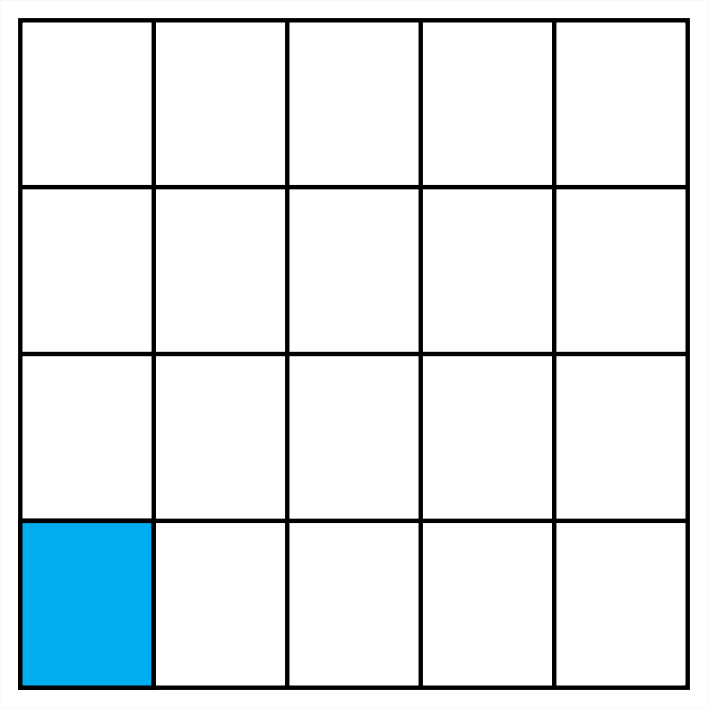
\includegraphics[width=45px]{../images/imagen_frac11.png} \fillin[\fbox{$\dfrac{1}{20}$}][0in] \\[1em]
			\end{parts}
		\end{multicols}
	}


   % \subsection*{\ifprintanswers{Nombre de fracciones                       }\else{}\fi}
	
   \questionboxed[5]{Escribe la fracción que corresponda en cada inciso:

		\begin{parts}
			\part ¿Cómo se escribe numéricamente la fracción \textbf{ocho quintos}?    \fillin[$\dfrac{8}{5}$][0in]  \\
			\part ¿Cómo se escribe numéricamente la fracción \textbf{seis onceavos}?   \fillin[$\dfrac{6}{11}$][0in] \\
			\part ¿Cómo se escribe numéricamente la fracción \textbf{dos séptimos}?    \fillin[$\dfrac{2}{7}$][0in]  \\
			\part ¿Cómo se escribe numéricamente la fracción \textbf{once medios}?     \fillin[$\dfrac{11}{2}$][0in] \\
			\part ¿Cómo se escribe numéricamente la fracción \textbf{diez décimos}?    \fillin[$\dfrac{10}{10}$][0in]\\
		\end{parts}
	}
   
   % \subsection*{\ifprintanswers{Conversión de fracciones mixtas a impropias}\else{}\fi}
	
   \questionboxed[3]{Convierte la siguientes fracciones mixtas a impropias:

		\begin{multicols}{3}
			\begin{parts}\large
				\part $4\dfrac{2}{3}= $ \fillin[$\dfrac{14}{3}$][0in]
				\part $2\dfrac{3}{10}= $ \fillin[$\dfrac{23}{10}$][0in]
				\part $5\dfrac{1}{5}= $ \fillin[$\dfrac{26}{5}$][0in]
			\end{parts}
		\end{multicols}
	}
   
   % \subsection*{\ifprintanswers{Conversión de fracciones impropias a mixtas}\else{}\fi}
	
   \questionboxed[3]{Convierte la siguientes fracciones impropias a mixtas:

		\begin{multicols}{3}
			\begin{parts}\large
				\part $\dfrac{13}{3}= $ \fillin[$4\dfrac{1}{3}$][0in]
				\part $\dfrac{63}{10}= $ \fillin[$6\dfrac{3}{10}$][0in]
				\part $\dfrac{51}{5}= $ \fillin[$10\dfrac{1}{5}$][0in]
			\end{parts}
		\end{multicols}
	}
   
   % \section*{\ifprintanswers{Operaciones con fracciones                 }\else{}\fi}
	% \subsection*{\ifprintanswers{Suma de fracciones                         }\else{}\fi}
	% \subsection*{\ifprintanswers{Resta de fracciones                        }\else{}\fi}
	% \subsection*{\ifprintanswers{Multiplicación de fracciones               }\else{}\fi}
	% \subsection*{\ifprintanswers{División de fracciones                     }\else{}\fi}
	% \subsection*{\ifprintanswers{Operaciones de fracciones mixtas           }\else{}\fi}

   \questionboxed[8]{Realiza las siguientes operaciones.

		\begin{multicols}{2}
			\begin{parts}\large
				\part $\dfrac{3}{10}+\dfrac{4}{5}=$ \fillin[$\dfrac{11}{10} = 1\dfrac{1}{10}$][0in] \\[0.75em]
				\part $\dfrac{3}{4}-\dfrac{2}{5}=$ \fillin[$\dfrac{7}{20}$][0in] \\[0.75em]
				\part $\dfrac{2}{3}-\dfrac{2}{5}=$ \fillin[$\dfrac{4}{15}$][0in] \\[0.75em]
				\part $\dfrac{3}{8}+\dfrac{7}{10}=$ \fillin[$\dfrac{43}{40} = 1\dfrac{3}{40}$][0in] \\[0.75em]
				\part $\dfrac{3}{5}\times\dfrac{2}{3}=$ \fillin[$\dfrac{6}{15}$][0in]   \\[0.75em]
				\part $\dfrac{7}{8}\times\dfrac{3}{4}=$ \fillin[$\dfrac{21}{32}$][0in] \\[0.75em]
				\part $\dfrac{3}{5} \divisionsymbol\dfrac{2}{3}=$ \fillin[$\dfrac{9}{10}$][0in] \\[0.75em]
				\part $\dfrac{7}{8} \divisionsymbol\dfrac{3}{4}=$ \fillin[$\dfrac{28}{24}$][0in]	\\[0.75em]
			\end{parts}
		\end{multicols}
	}
\end{questions}
\end{document}